% git-for-Rworkshop.tex - using slides from other talks to give 30 minute
%  Introduction to Git/GitHub at PBS R workshop.
\documentclass[aspectratio=169]{beamer}
%% For 4:3 aspect ratio:
%% \documentclass{beamer}
\usepackage{../git-course}

\title[git-course]{Introduction to Git and \gh}
\author{Andrew Edwards \& Chris Grandin}
\date{\today}

\begin{document}
%% Needed to remove 'Figure:' from figure captions:
\setbeamertemplate{caption}{\raggedright\insertcaption\par}

\frame[plain]{
\titlepage
}

\section{Introduction}

\frame{\frametitle{Motivation}
  \bi
    \item We are working far more collaboratively than in the past -- sharing code and writing documents.
    \item Stock assessments, for example, can be extremely complex with Bayesian output (recent Pacific Ocean Perch assessment had $>200$ figures in just one Appendix).
    \item How to share code and make sure we are working on the same version?
    \item Emailing versions of files back and forth is:
    \bi 
      \item very inefficient,
      \item prone to errors,
      \item painful.
    \ei
    \item With complex code we need to have {\red identical} folder structures on each other's computers.
  \ei
}

\frame{\frametitle{Definitions}
  \bi
    \item {\red Git} allows you to continually save the latest versions
       of your files (e.g. R code) as you work on them (`version control').
    \item It also allows you to go back to any previous version of your files.
    \item {\red GitHub} is a website that hosts a copy of the code and enables
       users to easily collaborate.
    \item We use these to collaborate when writing code and producing documents 
       (such as stock assessments), and to easily share code with others.
  \ei
}

\section{Avoid}
\frame{\frametitle{Examples of what we can avoid}

  \centering
  \begin{figure}
    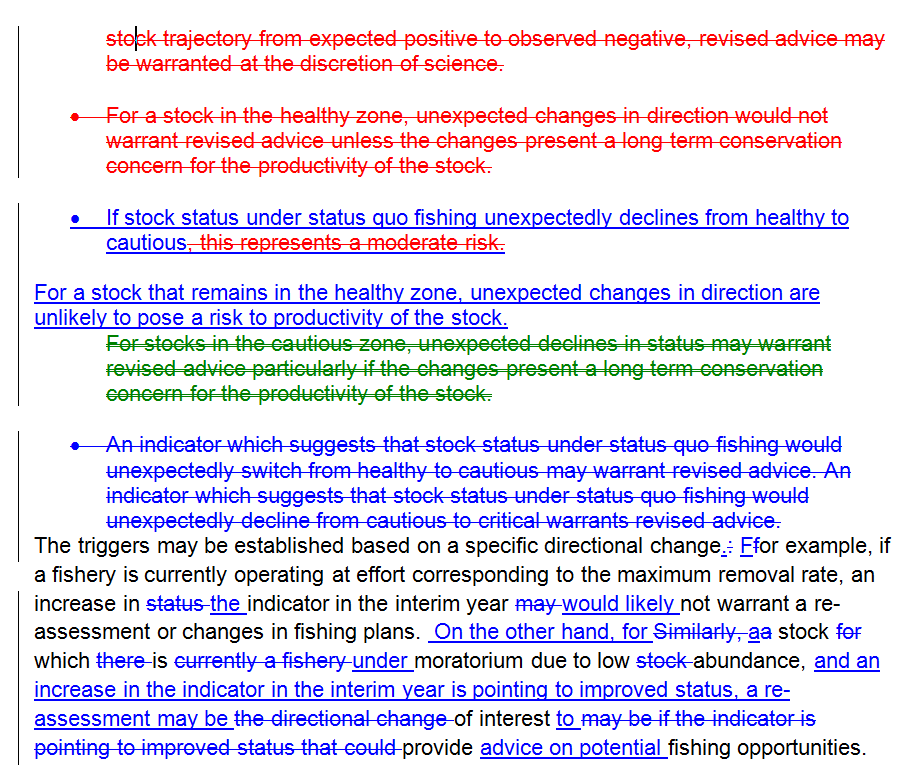
\includegraphics[
        width=\textwidth,
        height=0.8\textheight,
        keepaspectratio]
        {../git-motivation/figures/interim.png}
  %\vspace{-3mm}
  %\caption{\tiny\url{https://www.reddit.com/user/NegativePitch}}
  \end{figure}
}

\frame{\frametitle{Relying on one person (e.g.~me) who holds up a project}

  Often we may be collaborating on a project but be busy on something else, yet our collaborator has time.

  \centering
  \begin{figure}
    
\includegraphics[
        width=\textwidth,
        height=0.8\textheight,
        keepaspectratio]
        {../git-motivation/figures/procEmail.png}
  %\vspace{-3mm}
  %\caption{\tiny\url{https://www.reddit.com/user/NegativePitch}}
  \end{figure}
}

\frame{\frametitle{Cluttering up directories}

  We may want to keep old versions in case we have to go back, but then ...

  \centering
  \begin{figure}
    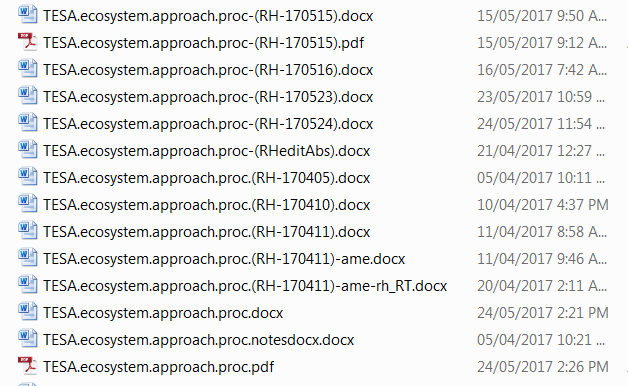
\includegraphics[
        width=\textwidth,
        height=0.8\textheight,
        keepaspectratio]
        {../git-motivation/figures/EAversions.png}
  \end{figure}
}

\frame{\frametitle{Can work simultaneously on same document (and then merge)}

  Can all keep up with the latest version (checking and merging each 
  other's work along the way), rather than ...

  \centering
  \begin{figure}
    
\includegraphics[
        width=\textwidth,
        height=0.8\textheight,
        keepaspectratio]
        {../git-motivation/figures/proposalEmail.png}
  \end{figure}
}

\section{\gh\ advantages}

\frame{\frametitle{Can easily catch up with collaborator}

  Chris did a lot of work (`commits') from 11th May ...

  ~\\
  ~\\
  \includegraphics[
     width=\textwidth,
     height=0.6\textheight,
     keepaspectratio]
     {../git-motivation/figures/netWorkGraph1}
}

\frame{\frametitle{Can easily catch up with collaborator}

  ... to 30th May:
  ~\\
  ~\\

  \includegraphics[
     width=\textwidth,
     height=0.6\textheight,
     keepaspectratio]
     {../git-motivation/figures/netWorkGraph2}

  I did nothing in that time ... 

}

\frame{\frametitle{Can easily catch up with collaborator}

  ... but just needed three commands (that you'll learn) to get caught up:
  ~\\
  ~\\

  \includegraphics[
     width=\textwidth,
     height=0.6\textheight,
     keepaspectratio]
     {../git-motivation/figures/netWorkGraph3}

  ~\\
  All files that Chris edited got updated, plus I now have any new files he created, and our folder structures are identical. 
}

\frame{\frametitle{Easy to answer other's questions}

  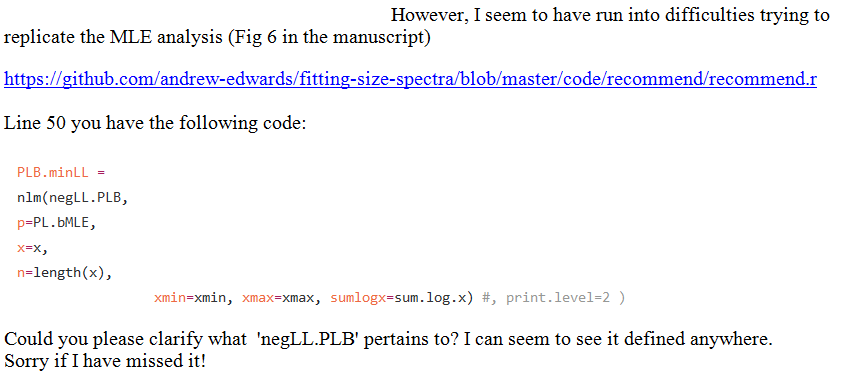
\includegraphics[
     width=\textwidth,
     height=0.80\textheight,
     keepaspectratio]
     {../git-motivation/figures/MEEcodeQuest}


  Rather than go to the code on my laptop that I haven't looked at for six months, I could click on link and answer very quickly.
}

\frame{\frametitle{Easy to answer other's questions}

  
\includegraphics[
     width=\textwidth,
     height=0.80\textheight,
     keepaspectratio]
     {../git-motivation/figures/MEEcodeAnswer}

~\\
  Can provide a clear answer with a link to the file I'm talking about. No ambiguity.
}

\frame{\frametitle{Hake assessment}

  \bi 
    \item Collaboration between four/five US and Canadian scientists.
    \item Annual assessment.
    \item Full Bayesian statistical catch-at-age model (complex output).
    \item Short turnaround between getting final data and submitting assessment.
    \item Short turnaround between review meeting and publishing assessment (two days).
    \item 2015 and before -- lots of editing and amalgamating Word files late at night. 
  \ei
}

\frame{\frametitle{Hake assessment}
  \bi
    \item After running models we can now automatically generate full document, including all numbers, figures and tables (via knitr and latex, all shared on \gh).

    \item Was a lot of work in 2016 to set up, but 2017 was way less stressful and resulted in more polished document.
    \item Praise on Twitter from one of the reviewers!      
  \ei
  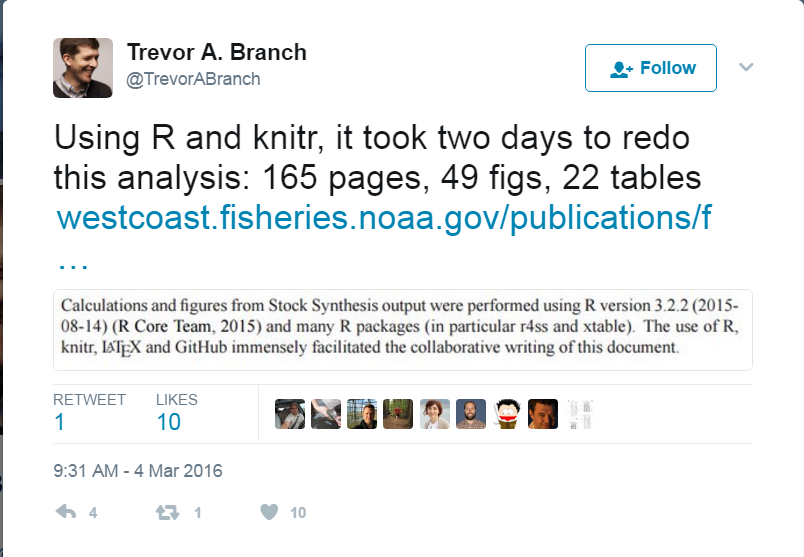
\includegraphics[
     width=\textwidth,
     height=0.50\textheight,
     keepaspectratio]
     {../git-motivation/figures/trevorTweet}
}

\frame{\frametitle{Who wrote that piece of garbage?}

  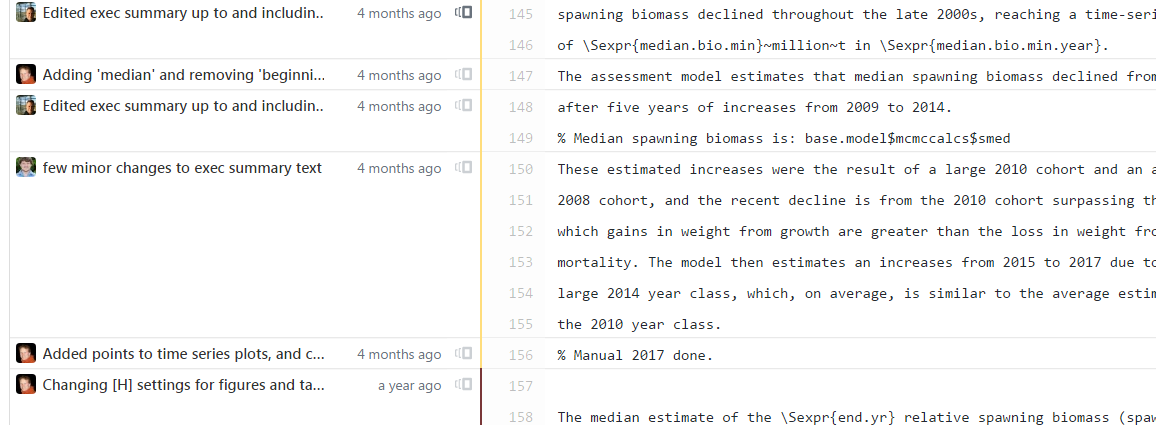
\includegraphics[
     width=\textwidth,
     height=0.80\textheight,
     keepaspectratio]
     {../git-motivation/figures/blame}

~\\
  Can be useful [on \gh: Code -- $<$click file$>$ -- Blame].
}

\frame{\frametitle{Can properly keep track of (and discuss) issues}

Rather than lots of emails that get forgotten, the to-do list actually gets completed.

  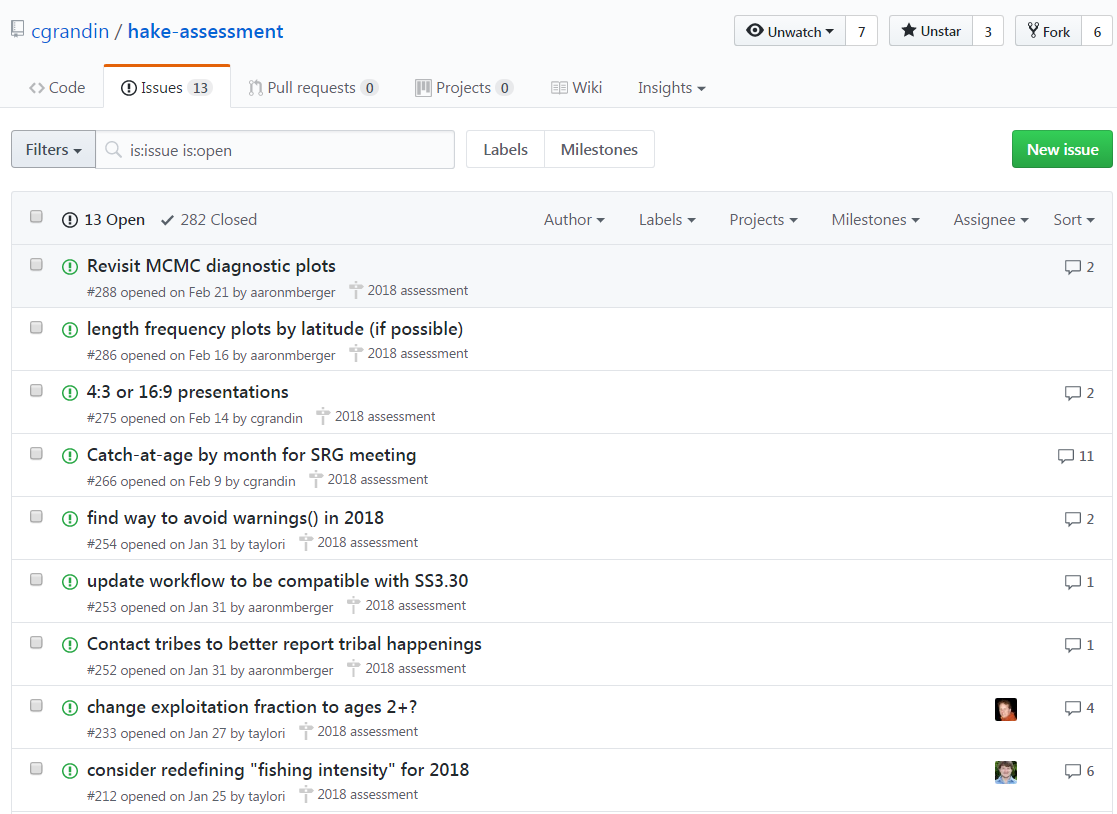
\includegraphics[
     width=\textwidth,
     height=0.80\textheight,
     keepaspectratio]
     {../git-motivation/figures/hakeIssues}
}

\frame{\frametitle{Can properly keep track of (and discuss) issues}

And you don't have to follow up with co-authors (who do have it under control):

~\\
  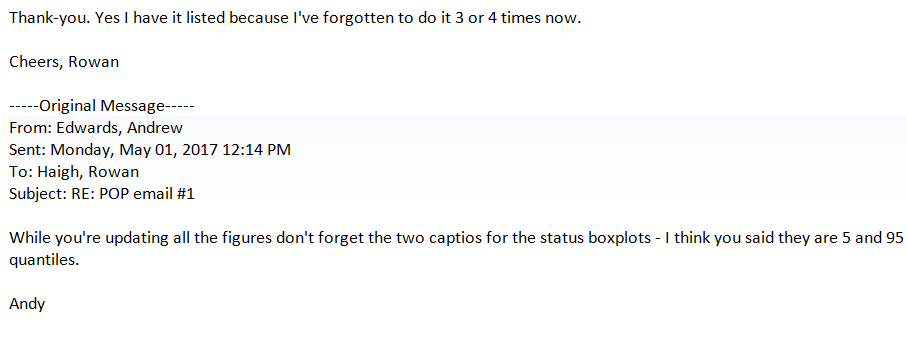
\includegraphics[
     width=\textwidth,
     height=0.80\textheight,
     keepaspectratio]
     {../git-motivation/figures/captionEmail}
}

\frame{\frametitle{Hake assessment}
  \bi
    \item For hake assessment:
      \url{https://github.com/andrew-edwards/hake-assessment/network}\\
    \item What's been happening recently?\\
    \item Scroll back to show some complexity.\\
    \item Click on `Contributors'.
  \ei
}

\section{Summary}

\frame{\frametitle{Summary}

  \bi
    \item Ideal for sharing of R code.
    \item `Repositories' can be public or private.
    \item Caveat -- cannot (properly) collaborate on Word files.
    \item BUT there's a way of converting Markdown using pandoc to generate a Word file.
    \item Hake example is to show how far you can get.
    \item There is a learning curve, but once you use \gh\ you only really need a few main commands.
  \ei
}

\section{Demonstration}

\frame{\frametitle{Demonstration using code that builds these slides}
  \bi
    \item Idea is the same as if this was R code.
    \item These slides are part of our \lst{git-course} repository.
    \item I worked on these since our workshop last week. Chris had been
      busy on other projects and so yesterday (Tues 27th) his Network Graph
      looked like this:
  \ei
  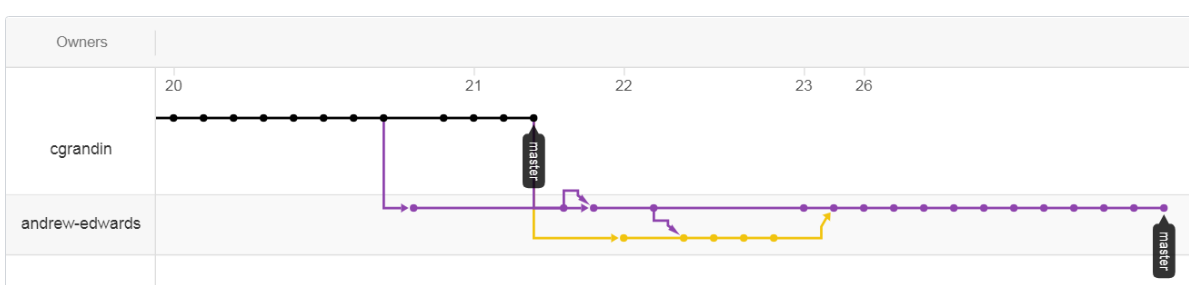
\includegraphics[
     width=\textwidth,
     height=0.80\textheight,
     keepaspectratio]
     {figures/NGbeforeCmerges}
}


\frame{\frametitle{Demonstration on code that builds these slides}
  \bi
    \item This morning (Wed 27th) Chris has made some changes, added files etc.
    \item I will show how easy it is to \lst{fetch} and then \lst{merge} his
      edits.
    \item I will re-run the code to build these slides.
    \item This workflow is the same as if were working together on R code, 
      including multiple files spread across several folders. 
    \item We can both work on the same files.
    \item Occasionally we will get a {\red conflict} -- we have both edited
      the same lines of the same file.
    \item This can be easily rectified and we can carry on.
  \ei
}

\frame{\frametitle{Can even jump back to any earlier version}
  \bi
    \item I can easily go back to any earlier version.
    \item For example, go back to before I got Chris's code and before
      I finished this slide.
    \item {\red This is the version before I finished this slide}
  \ei
}

\end{document}
